\documentclass[runningheads]{llncs}

\usepackage[T1]{fontenc}
\usepackage[utf8]{inputenc}
\usepackage{graphicx}
\usepackage{booktabs}
\usepackage{amsmath}
\usepackage{url}

\begin{document}

\title{Large vs.\ Small LLMs as Evaluators of\\ Abstractive Summarization}

\author{\"Umit Arslan}
\institute{Department of Computer Engineering,\\
Izmir Institute of Technology, Izmir, T\"urkiye\\
\email{umtarsln0@gmail.com}}

\maketitle

\begin{abstract}
Large language models (LLMs) are increasingly used as automatic \emph{judges} of
text-generation quality because they align with human judgements far better than
n-gram or embedding metrics. The strongest judges, however, are large and costly.
We ask a practical question for abstractive summarization: how much evaluation
quality is lost when a \emph{small, open} LLM judge replaces a \emph{large} one?
Using a single LLM-as-a-judge pipeline, we score summaries from the SummEval
benchmark on four dimensions---faithfulness, coherence, relevance and
fluency---with a small open judge (Qwen2.5-3B, run locally) and a large proprietary
judge (Google Gemini 2.5 Flash), each using an identical rubric and chain-of-thought
prompt. We
compare both against three baselines (ROUGE, BERTScore and a rubric-free zero-shot
variant of the small model) on how well their scores correlate with human ratings,
how closely the two judges agree, and their cost and speed. The large judge
correlates with human ratings far better than every baseline (average Spearman
$0.50$ vs.\ at most $0.26$), but the small judge does \emph{not}: at $0.21$ it is
statistically indistinguishable from ROUGE and BERTScore and, strikingly, no better
than its own rubric-free zero-shot variant---a rubric and chain-of-thought help the
large model but not the small one. The small judge also shows a severe strictness
bias, scoring up to $2.5$ points lower than the large judge on faithfulness. We
conclude that, on this benchmark, a small open judge is not yet a drop-in
replacement for a large one; it offers only a cheap, rough signal. We report
bootstrap confidence intervals throughout and release all code and prompts for
reproducibility.

\keywords{LLM-as-a-judge \and summarization evaluation \and SummEval \and
chain-of-thought \and small language models.}
\end{abstract}

\section{Introduction}

Automatic evaluation of generated text is a long-standing bottleneck in natural
language generation. For abstractive summarization, lexical-overlap metrics such as
ROUGE~\cite{lin2004rouge} and embedding-based metrics such as
BERTScore~\cite{zhang2020bertscore} are cheap and reproducible, but they correlate
only weakly with human judgements of qualities such as factual consistency or
coherence~\cite{fabbri2021summeval}. The ``LLM-as-a-judge'' paradigm---prompting a
strong language model to rate or compare outputs---has emerged as a much stronger
alternative, matching human preferences closely on a range of
tasks~\cite{zheng2023judging,liu2023geval,fu2023gptscore}. The catch is that the
best judges are large, often proprietary, models that are expensive, rate-limited
and difficult to reproduce.

This motivates a simple, practical question:

\begin{quote}
\emph{Does replacing a large LLM judge with a small, open one meaningfully hurt
evaluation quality, and by how much?}
\end{quote}

This is an \emph{evaluation} study, not a generation study: the system never writes
summaries. It scores summaries that already exist in the SummEval
benchmark~\cite{fabbri2021summeval} and measures how well those scores track human
ratings. We instantiate one LLM-as-a-judge pipeline and run it with two judges of
very different size and access model---a small open judge, Qwen2.5-3B~\cite{qwen2025}
served locally, and a large proprietary judge, Google Gemini 2.5
Flash~\cite{gemini2024}, accessed through its API---under an identical rubric and
chain-of-thought (CoT) prompt~\cite{wei2022chain}. Both are compared with
three baselines: ROUGE, BERTScore, and a rubric-free zero-shot scoring variant of
the small model that isolates the contribution of prompt design.

\paragraph{Contributions.} (1) A controlled comparison of a small open vs.\ a large
proprietary LLM judge for summarization, holding the prompt, dataset and parsing fixed. (2) A
three-way analysis---human alignment, judge--judge agreement, and cost/speed---with
bootstrap confidence intervals to account for the modest subset size. (3) A fully
open, reproducible pipeline (local small judge via Ollama; committed prompts, seeds
and code).

\section{Related Work}

\paragraph{Reference-based metrics.} ROUGE~\cite{lin2004rouge} measures n-gram
overlap with reference summaries and remains a default in summarization.
BERTScore~\cite{zhang2020bertscore} replaces surface overlap with similarity between
contextual BERT embeddings, improving correlation with human judgement. Both are
\emph{reference-based}: they compare a candidate to gold summaries rather than
judging it against the source, which limits their sensitivity to faithfulness.

\paragraph{Meta-evaluation of summarization.} SummEval~\cite{fabbri2021summeval}
re-evaluated summarization metrics on outputs of modern systems for CNN/DailyMail
articles, collecting expert annotations along coherence, consistency, fluency and
relevance. It showed that many automatic metrics correlate weakly with human scores
and provides the human ratings we use as ground truth.

\paragraph{LLMs as judges.} G-Eval~\cite{liu2023geval} uses GPT-4~\cite{openai2023gpt4}
with chain-of-thought and a form-filling protocol, reaching far higher human
correlation than prior metrics. GPTScore~\cite{fu2023gptscore} frames evaluation as
the model's likelihood of a quality-conditioned continuation. Zheng et
al.~\cite{zheng2023judging} study LLM judges for open-ended chat, documenting strong
agreement with humans alongside biases (position, verbosity, self-enhancement).
Most of this work relies on large proprietary models such as
GPT-4~\cite{openai2023gpt4} or Gemini~\cite{gemini2024}. We focus instead on whether
a \emph{small open} model can stand in for a large one, which determines whether
LLM-based evaluation is affordable and reproducible at scale.

\section{Methodology}

\subsection{Task Formulation}
Given a source document $d$, a machine summary $s$ and a scoring rubric, a judge
produces four integer scores in $\{1,\dots,5\}$ for \emph{faithfulness},
\emph{coherence}, \emph{relevance} and \emph{fluency}. We treat the judge's
faithfulness score as the counterpart of SummEval's \emph{consistency} dimension
(factual consistency with the source); the other three names align directly. We do
not generate summaries; we only score existing ones and correlate the scores with
human ratings.

\subsection{Judges}
Both judges receive an identical prompt and decode at temperature~0 for
deterministic scores. The \textbf{small judge} is Qwen2.5-3B-Instruct~\cite{qwen2025},
an open model run locally through an Ollama server (4-bit quantization) on a single
consumer GPU---representing the cheap, reproducible regime. The \textbf{large judge}
is Google Gemini 2.5 Flash~\cite{gemini2024}, a large proprietary model accessed
through its API, matching the proposal's intent of contrasting a small local judge
with a large proprietary one. The variable of interest is the judge's
\emph{scale and capability}.

\subsection{Rubric and Chain-of-Thought Prompt}
A single prompt template defines the four dimensions, instructs the model to reason
briefly (2--4 sentences) before scoring, and to emit a final JSON object with the
four integer scores. Chain-of-thought reasoning~\cite{wei2022chain} before the
numeric verdict is the key prompt-design element shared by both judges; the prompt
is identical across judges and committed verbatim in the repository.

\subsection{Baselines}
\textbf{ROUGE}~\cite{lin2004rouge} (ROUGE-1/2/L F-measure, max over references) and
\textbf{BERTScore}~\cite{zhang2020bertscore} (F, RoBERTa-large) are reference-based.
\textbf{Zero-shot Direct Scoring} uses the \emph{same} small model prompted for a
single overall 1--5 score with no rubric and no reasoning; comparing it with the
rubric+CoT small judge isolates how much of the small judge's quality comes from
prompt design rather than raw model ability.

\subsection{Output Parsing}
Small models occasionally emit malformed output. The judge output is parsed by first
extracting the trailing JSON object and, failing that, a per-dimension regular
expression; up to two re-queries are issued before a record is marked unparsed.
This structured-output-plus-fallback strategy keeps parse failures negligible.

\section{Experimental Setup}

\subsection{Dataset}
We use SummEval~\cite{fabbri2021summeval} (the \texttt{mteb/summeval} release, 100
articles, each with 16 machine summaries and expert human ratings on the four
dimensions). We build a fixed, seeded evaluation subset of all 100 articles,
sampling 8 of the 16 machine summaries per article, yielding 800 summary-level
records. The subset is regenerated deterministically from a fixed seed.

\subsection{Metrics}
Human alignment is measured by Spearman's $\rho$ and Kendall's $\tau$ between each
method's scores and the human ratings, per dimension and averaged. For the two LLM
judges each dimension is matched to its human counterpart; the single-value methods
(ROUGE, BERTScore, zero-shot) are correlated against each human dimension, as is
standard for reference metrics. Judge--judge agreement is measured by Pearson
correlation and the mean (signed and absolute) score difference. Because the subset
is modest, we report \textbf{95\% bootstrap confidence intervals} (1000 resamples
over records) for the average correlations. Cost is reported as tokens per summary,
latency and throughput.

\subsection{Implementation Details}\label{sec:impl}
The small judge and zero-shot baseline run on Qwen2.5-3B via Ollama; the large judge
runs on Gemini 2.5 Flash via the Google Gemini API with client-side rate limiting. BERTScore runs on CPU
to avoid contending with the local judge for GPU memory. Long source bodies are
lightly truncated to fit the small model's context window. All decoding uses
temperature~0; seeds, prompts and pinned dependencies are committed. Each stage
writes its scores to disk so later stages and analyses are fully reproducible from
the released artifacts.

\section{Results}

\begin{table}[t]
\centering
\caption{Spearman correlation of each method with SummEval human ratings, per dimension. Avg.\ columns report the mean Spearman ($\rho$) and Kendall ($\tau$) across the four dimensions. LLM judges in bold.}
\label{tab:correlation}
\begin{tabular}{lcccccc}
\toprule
Method & Coh. & Cons. & Flu. & Rel. & Avg.\,$\rho$ & Avg.\,$\tau$ \\
\midrule
ROUGE-1 & 0.214 & 0.186 & 0.102 & 0.313 & 0.204 & 0.151 \\
ROUGE-2 & 0.144 & 0.150 & 0.076 & 0.221 & 0.148 & 0.109 \\
ROUGE-L & 0.212 & 0.153 & 0.078 & 0.230 & 0.168 & 0.124 \\
BERTScore-F & 0.385 & 0.075 & 0.092 & 0.373 & 0.231 & 0.169 \\
Zero-shot & 0.296 & 0.238 & 0.232 & 0.278 & 0.261 & 0.226 \\
\textbf{Small judge} & 0.244 & 0.261 & 0.128 & 0.210 & 0.210 & 0.183 \\
\textbf{Large judge} & 0.506 & 0.621 & 0.417 & 0.452 & 0.499 & 0.434 \\
\bottomrule
\end{tabular}
\end{table}

\begin{table}[t]
\centering
\caption{Average human Spearman correlation with 95\% bootstrap confidence intervals (1000 resamples over the evaluation records).}
\label{tab:bootstrap}
\begin{tabular}{lcc}
\toprule
Method & Avg.\ Spearman & 95\% CI \\
\midrule
ROUGE-1 & 0.204 & [0.156, 0.251] \\
ROUGE-2 & 0.148 & [0.094, 0.195] \\
ROUGE-L & 0.168 & [0.120, 0.216] \\
BERTScore-F & 0.231 & [0.185, 0.281] \\
Zero-shot & 0.261 & [0.212, 0.311] \\
Small judge & 0.210 & [0.171, 0.250] \\
Large judge & 0.499 & [0.459, 0.536] \\
\bottomrule
\end{tabular}
\end{table}

\begin{table}[t]
\centering
\caption{Agreement between the small and large judge per dimension: Pearson correlation, mean signed difference (small$-$large; negative means the small judge is stricter) and mean absolute difference.}
\label{tab:agreement}
\begin{tabular}{lccc}
\toprule
Dimension & Pearson & Mean diff. & Mean abs.\ diff. \\
\midrule
Faithfulness & 0.337 & -2.473 & 2.527 \\
Coherence & 0.194 & -1.653 & 1.767 \\
Relevance & 0.232 & -0.762 & 1.046 \\
Fluency & 0.208 & -1.294 & 1.413 \\
Overall & 0.221 & -1.546 & 1.688 \\
\bottomrule
\end{tabular}
\end{table}

\begin{table}[t]
\centering
\caption{Cost and speed of the model-based methods on the evaluation subset.}
\label{tab:cost}
\begin{tabular}{lccccc}
\toprule
Method & $N$ & Tok./summ. & Lat.\ (s) & Summ./min & Monetary \\
\midrule
Zero-shot (local) & 800 & 615 & 0.85 & 70.1 & \$0 (local GPU) \\
Small judge (local) & 800 & 1122 & 6.20 & 9.7 & \$0 (local GPU) \\
Large judge (Gemini) & 800 & 931 & 1.10 & 54.6 & $\sim$\$0.40 \\
\bottomrule
\end{tabular}
\end{table}


\subsection{Human Alignment}
Table~\ref{tab:correlation} reports per-dimension and average Spearman/Kendall
correlations with human ratings, Table~\ref{tab:bootstrap} the average Spearman with
95\% bootstrap confidence intervals, and Fig.~\ref{fig:bars} the average alignment.
The \textbf{large judge} is the clear winner: it has the highest correlation on every
dimension and an average Spearman of $0.50$---roughly double the best baseline---with
a confidence interval ($[0.46, 0.54]$) that does not overlap any other method. It is
strongest on consistency/faithfulness ($\rho=0.62$), precisely the dimension that
reference metrics capture worst.

The \textbf{small judge} tells a very different story. Its average correlation
($0.21$) is statistically indistinguishable from ROUGE-1 ($0.20$) and BERTScore
($0.23$)---the confidence intervals overlap almost entirely---so rubric-guided
judging by a 3B model buys essentially nothing over cheap reference metrics here.
More strikingly, the small \emph{rubric+CoT} judge ($0.21$) is no better than, and in
point estimate slightly below, the \emph{rubric-free} zero-shot variant of the same
model ($0.26$). The elaborate rubric and chain-of-thought that help the large model
therefore do \emph{not} help the small one: a 3B model scores summaries about as well
with a bare ``rate 1--5'' prompt. On this benchmark, human alignment is driven far
more by judge \emph{scale} than by prompt design.

\begin{figure}[t]
\centering
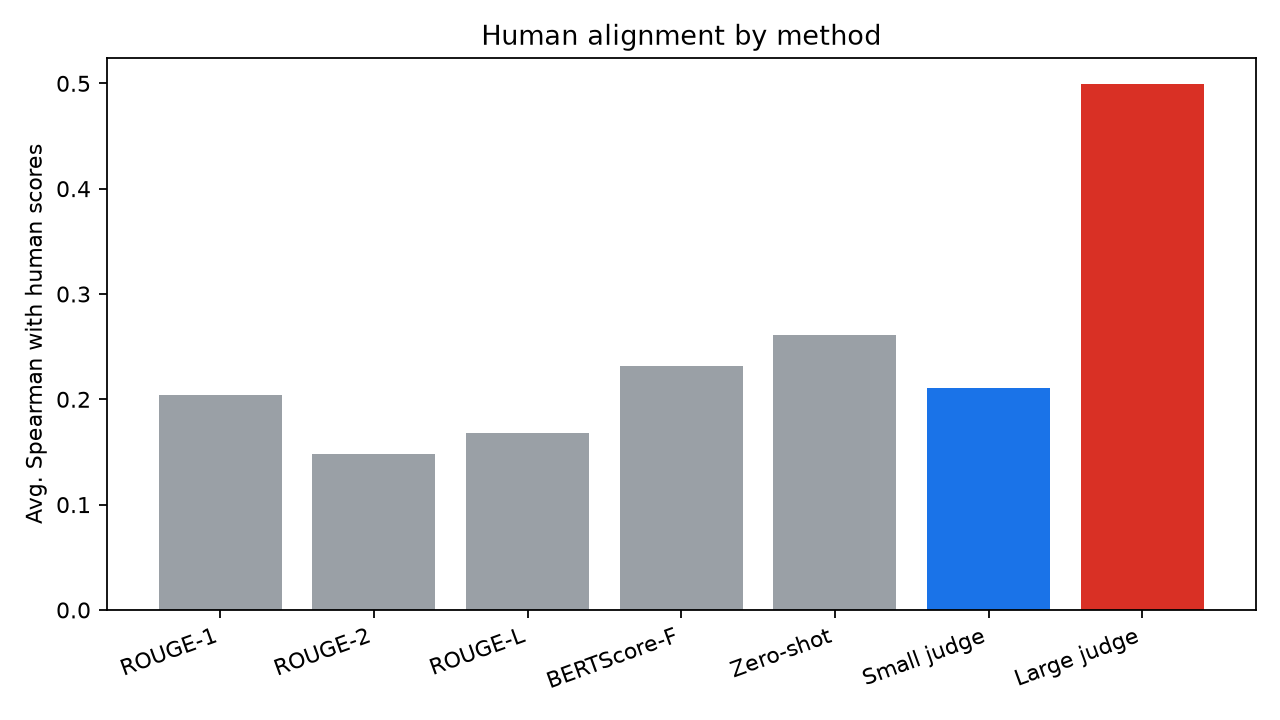
\includegraphics[width=0.78\textwidth]{correlation_bars.png}
\caption{Average Spearman correlation with human ratings by method. The large judge
(red) dominates every method, while the small judge (blue) is only on par with the
reference-based and zero-shot baselines.}
\label{fig:bars}
\end{figure}

\subsection{Judge--Judge Agreement}
Table~\ref{tab:agreement} reports agreement between the two judges. Their scores
correlate only weakly (overall Pearson $0.22$), and the small judge is systematically
and substantially \emph{stricter}: it scores about $1.5$ points lower than the large
judge on average, rising to $2.5$ points on faithfulness, where it assigns low scores
even to summaries the large judge and human annotators consider consistent. This
large, systematic strictness/compression bias---not random noise---is the small
judge's dominant failure mode. Because it is systematic, simple score
\emph{calibration} (e.g.\ per-judge standardisation) is a plausible partial remedy,
though it cannot recover rank information the small judge never produced.

\subsection{Cost and Speed}
Table~\ref{tab:cost} summarises the cost--quality trade-off, and the two regimes
differ sharply. The small judge runs entirely locally at zero API
cost but is slow on a consumer GPU ($\sim$6\,s per summary, $9.7$ summaries/min). The
large judge, on a paid but inexpensive API, is both faster ($\sim$1\,s per summary)
and far more accurate, costing only about US\$0.40 for all $800$ summaries
($\sim$US\$0.0005 each). On this benchmark the large judge therefore dominates on
quality at a near-trivial price; the small judge's appeal is confined to settings
where local execution or zero marginal cost outweighs a large loss in evaluation
quality.

\section{Discussion}
Our results give a clear, and largely negative, answer to the motivating question. On
SummEval, replacing a large judge with a small open one does \emph{not} merely cost a
little quality---it erases most of the benefit of LLM-as-a-judge: the small judge's
human alignment ($0.21$) falls back to the level of the ROUGE/BERTScore baselines it
was meant to surpass, while the large judge ($0.50$) stands well above everything.
Two findings sharpen this picture. First, rubric and chain-of-thought
prompting---central to methods such as G-Eval~\cite{liu2023geval}---are \emph{not}
model-agnostic: they help the large judge but give the 3B model no advantage over a
bare direct score, suggesting the small model lacks the capacity to exploit the
structured protocol. Second, the small judge's errors are dominated by a large,
systematic strictness bias rather than random noise, which calibration can dampen but
not remove. For practitioners, the implication is that LLM-as-a-judge for
summarization currently hinges on judge scale: a small local judge gives a cheap,
rough signal, but trustworthy automatic evaluation still needs a large judge---which,
encouragingly, costs only cents per several hundred summaries.

\section{Limitations}
The evaluation subset, though seeded and spanning all SummEval articles, is modest;
we therefore report bootstrap confidence intervals, which are non-trivially wide and
should temper strong rankings. SummEval covers a single domain (CNN/DailyMail news).
Our large judge is Gemini 2.5 Flash, a capable but not frontier-scale model, and the
two judges differ in architecture and training as well as size, so the comparison
reflects a realistic small-open vs.\ large-proprietary contrast rather than a pure
parameter-count ablation; results may differ for the very largest judges such as
GPT-4~\cite{openai2023gpt4}. Light source truncation may remove information relevant
to faithfulness. Finally, scores at temperature~0 are
deterministic but do not capture sampling variance.

\section{Conclusion}
We compared a small open judge (Qwen2.5-3B, local) and a large proprietary judge
(Gemini 2.5 Flash) for abstractive-summarization evaluation under an identical rubric
and chain-of-thought prompt, against ROUGE, BERTScore and a rubric-free baseline, on
a seeded SummEval subset of $800$ summary-level records. The large judge correlates
with human ratings far better than every other method (average Spearman $0.50$), but
the small judge does not: at $0.21$ it is indistinguishable from the classical
metrics and no better than its own rubric-free variant, and it suffers a severe
strictness bias. The quality gap thus tracks judge scale, and prompt sophistication
does not close it. We conclude that a small open judge is not yet a drop-in
replacement for a large one in summarization evaluation, even though the large
judge's monetary cost is negligible. All code, prompts and configuration are released
for reproducibility.

\bibliographystyle{splncs04}
\bibliography{references}

\end{document}
